%% In the documentclass line, replace "noanswers" with "answers" to view the key.

\documentclass[noanswers]{exam}
\usepackage[utf8]{inputenc}

\title{Learning Activity 18}
\author{Chapter 10}
\date{STAT 3090}

\usepackage[bottom=2.2cm, left=2.2cm, right=2.2cm, top=2.2cm]{geometry}
%\usepackage[paperheight=11in, paperwidth=17in, margin=1in]{geometry}
\usepackage{dsfont}
\usepackage{amsmath}
\usepackage{amssymb}
\usepackage{amsthm}
\usepackage{array}
\usepackage{stmaryrd}
\usepackage{pgfplots}
\pgfplotsset{width=10cm,compat=1.9}
\usepackage{multicol}
\setlength{\columnsep}{1in}
\usepackage{nicefrac}

\usepackage{multirow}
\usepackage{enumitem}[shortlabels]
\usepackage{tabu}
\definecolor{purp}{RGB}{102,0,204}
\usepackage{tabularx}
\newcolumntype{C}{>{\centering\arraybackslash $}X<{$}}
\usepackage{wrapfig}
\usepackage[export]{adjustbox}


\makeatletter
\pagestyle{headandfoot}
\firstpageheader{\@date}{\@title}{\@author}
\firstpageheadrule
\runningfootrule
\runningfooter{}{\thepage\ / \numpages}{\@title}
\makeatother

\newcommand{\abs}[1]{\left|#1\right|}
\newcommand{\mat}[4]{\left( \begin{tabular}{>{$}c<{$} >{$}c<{$}} #1&#2 \\ #3&#4 \end{tabular} \right)}
\newcommand{\msc}[1]{\mathds{#1}}
\newcommand{\Z}{\mathds{Z}}
\newcommand{\R}{\mathds{R}}
\newcommand{\N}{\mathds{N}}
\newcommand{\Q}{\mathds{Q}}
\newcommand{\C}{\mathds{C}}
\newcommand{\so}{\implies}
\newcommand{\set}[2]{\left\{ #1 \:|\: #2 \right\}}
\newcommand{\bso}{\Longleftarrow}
\newcommand{\ra}{\rightarrow}
\newcommand{\gen}[1]{\left\langle #1 \right\rangle}
\newcommand{\olin}[1]{\overline{#1}}
\newcommand{\Img}[1]{\text{Im}\left(#1\right)}
\newcommand{\llra}{\longleftrightarrow}
\newcommand{\lra}{\longrightarrow}
\newcommand{\xra}[1]{\xrightarrow{#1}}
\newcommand{\wo}{\setminus}
\newcommand{\mcal}[1]{\mathcal{#1}}
\newcommand{\Aut}[1]{\text{Aut}\left(#1\right)}
\newcommand{\Inn}[1]{\text{Inn}\left(#1\right)}
\newcommand{\syl}[2]{\text{Syl}_{#1}(#2)}
\newcommand{\norm}[1]{\left\|#1\right\|}
\newcommand{\infnorm}[1]{\left\|#1\right\|_{\infty}}
\newcommand{\xn}{\{x_n\}}
\newcommand{\sig}{\sigma}
\newcommand{\id}{\text{id}}
\newcommand{\ep}{\epsilon}
\newcommand{\st}{\text{ s.t. }}
\newcommand{\ran}[1]{\text{Ran}(#1)}
\newcommand{\nCr}[2]{\binom{#1}{#2}}
\newcommand{\Exr}[1]{\paragraph{Exercise #1:}}
\newcommand{\pg}{\paragraph{}}
\newcommand{\ulin}[1]{\underline{#1}}
\newcommand{\tc}[1]{\textcolor{purp}{#1}}

% Solution Specs
\unframedsolutions
\renewcommand{\solutiontitle}{}
\SolutionEmphasis{\color{purp}}
\CorrectChoiceEmphasis{\color{purp}\bfseries}
\setlength\fillinlinelength{1.5in}
\renewcommand{\arraystretch}{2}


\begin{document}
\noindent\begin{tabular}{@{}p{1.4in}p{5.2in}@{}}
Group Member Names: & \hrulefill
\end{tabular}

\vspace{1mm}
\noindent If you have group members who collaborated but were not logged into the Zoom session, please note in the submission comments how they collaborated on the learning activity.

\vspace{5mm}

\noindent The manufacturers of Ramen noodles, a favorite college student staple, are interested in whether the variance of sodium levels in their product has \textbf{changed} after they began using different ingredients. With the old ingredients, the sodium levels of Ramen were determined to have a population standard deviation of 110 mg. A random sample of 20 packages made with the new ingredients was analyzed and found to have a sample standard deviation of 139.2~mg. Suppose that the sodium levels are normally distributed. Is there evidence at the $\alpha=0.10$ level that the variance of the sodium content has changed with the new ingredients?

\vspace{3mm}

\begin{questions}	
	
	\question Define the parameter in context and state your hypotheses.
		
	\begin{solution}[\stretch{1}]

	\vspace{1mm}
	
	$\sigma^2=$ the true variance in Ramen sodium levels using the new ingredients \textbf{\textit{\underline{or}}}
	
	$\sigma=$ the true standard deviation in Ramen sodium levels using the new ingredients
	
	\vspace{3mm}
	
	$H_0: \sigma^2=12,000$ \hspace{10mm} \textbf{\textit{\underline{or}}} \hspace{10mm} $H_0:\sigma=110$
	
	$H_1: \sigma^2\neq 12,000$\hspace{11mm} \textbf{\textit{\underline{or}}} \hspace{10mm} $H_1:\sigma\neq 110$
	
	\vspace{1mm}
	
	\end{solution}
	
	\question State and verify that the appropriate conditions for inference are met.
	
	\begin{solution}[\stretch{1}]
	
	\vspace{1mm}
	
	(1) The sample is randomly selected (stated).
	
	(2) The population of sodium levels are normally distributed.
	
	\vspace{1mm}	
	
	\end{solution}
	
	\question Compute the test statistic for this sample. Label it using the correct symbol.
	
	\begin{solution}[\stretch{1}]
	
	\vspace{1mm}
	
	$\chi_0^2=\displaystyle \frac{(20-1)(139.2)^2}{(110)^2}=30.43$
	
	\vspace{1mm}
	
	\end{solution}
	
	\question Find the critical values for the test and state the rejection region. \underline{Include a sketch} that shows the rejection region with the critical values on the horizontal axis and the appropriate areas shaded.
	
	\vspace{-5mm}
	
	\begin{solution}[\stretch{1}]
	
	\begin{multicols}{2}
	
	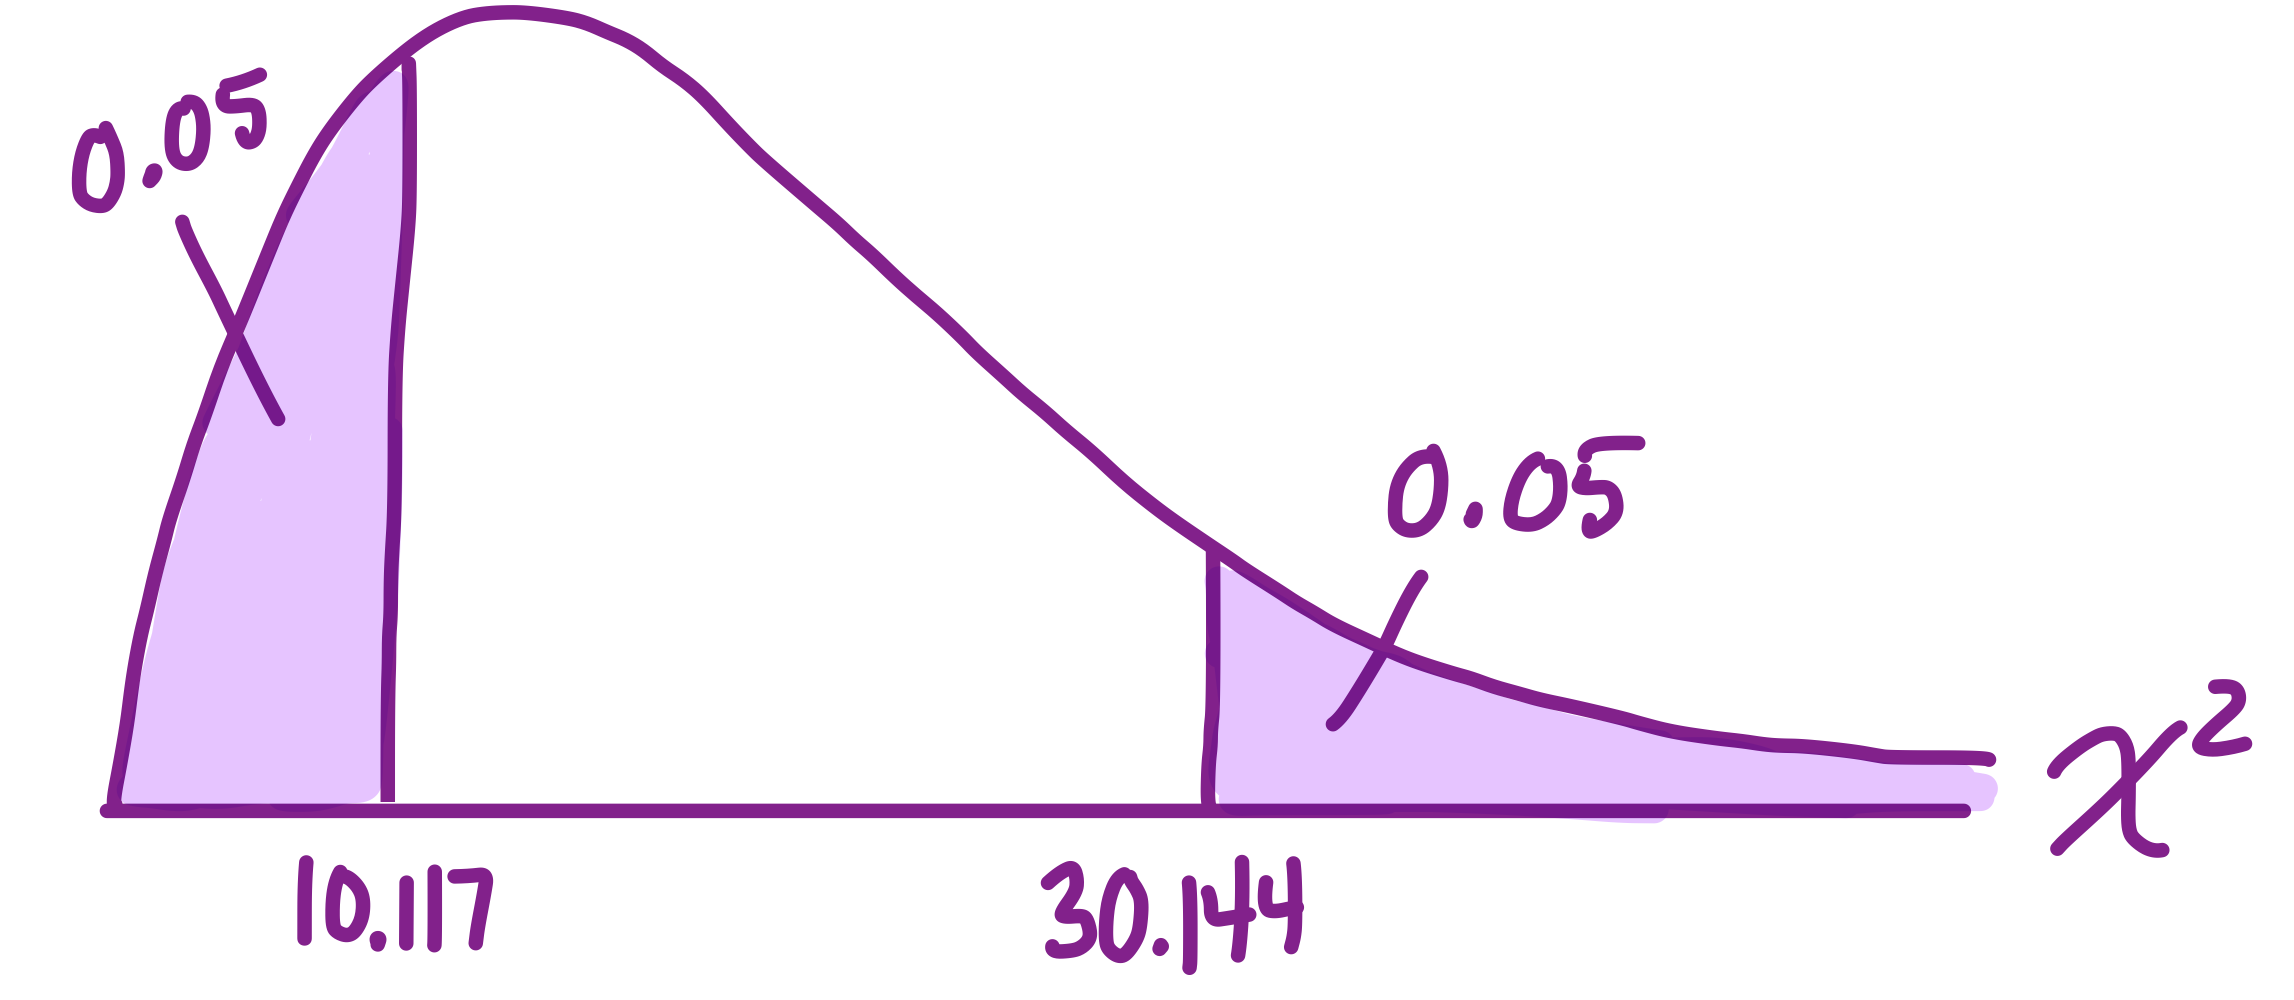
\includegraphics[scale=0.09]{STAT_3090_LA18_chisq.JPEG}
    
    $\alpha=0.10 \Rightarrow \nicefrac{\alpha}{2}=0.05$
	
	$df=20-1=19$
	
	$\chi_{.95,19}^2=10.117$
	
	$\chi_{.05,19}^2=30.144$
	
	RR: $\chi^2<10.117$ or $\chi^2>30.144$
	
	
	\end{multicols}

	\end{solution}	
	
	\question What is your decision about the null hypothesis? Provide support for your decision.
	
	\begin{solution}[\stretch{1}]
	
	\vspace{1mm}
	
	Because $\chi_0^2=30.53>30.144$ (i.e. the test statistic is in the rejection region), we reject $H_0$. 
	
	\vspace{1mm}
	
	\end{solution}
	
%	\newpage 
	
	\question Summarize the results of your test in context.
	
	\begin{solution}[\stretch{1}]
	
	\vspace{1mm}
	
	At the $\alpha=0.10$ level, we have sufficient evidence that...
	\begin{itemize}
	\item the true variance of Ramen sodium levels using the new ingredients is different than 12,100 mg$^2$.
	\item the true standard deviation of Ramen sodium levels using the new ingredients is different than 110 mg.
	\item the true variance / standard deviation of Ramen sodium levels has changed with the new ingredients.
	\end{itemize}
	(Any of the above would be correct.)
	\end{solution}
	
\end{questions}
%-----------------------------------------------------------------------------%

\end{document}
